\documentclass[final]{fhnwreport}       %[mode] = draft or final
                                        %{class} = fhnwreport, article, 
                                        %          report, book, beamer, standalone
%%---Main Packages-----------------------------------------------------------------------
\usepackage[english, ngerman]{babel}	%Mul­tilin­gual sup­port for LaTeX
\usepackage[T1]{fontenc}				%Stan­dard pack­age for se­lect­ing font en­cod­ings
\usepackage[utf8]{inputenc}				%Ac­cept dif­fer­ent in­put en­cod­ings
\usepackage{lmodern}                    %The newer Font-Set
\usepackage{textcomp}					%LaTeX sup­port for the Text Com­pan­ion fonts
\usepackage{graphicx} 					%En­hanced sup­port for graph­ics
\usepackage{float}						%Im­proved in­ter­face for float­ing ob­jects
\usepackage{ifdraft}                    %Let you check if the doc is in draft mode

%%---Useful Packages---------------------------------------------------------------------
\usepackage[pdftex,dvipsnames,table]{xcolor}  %Driver-in­de­pen­dent color ex­ten­sions for LaTeX
\usepackage{csquotes}                   %Simpler quoting with \enquote{}
\usepackage{siunitx} 					%A com­pre­hen­sive (SI) units pack­age
\usepackage{listings}					%Type­set source code list­ings us­ing LaTeX
\usepackage[bottom]{footmisc}			%A range of foot­note op­tions
\usepackage{footnote}					%Im­prove on LaTeX's foot­note han­dling
\usepackage{verbatim}					%Reim­ple­men­ta­tion of and ex­ten­sions to LaTeX ver­ba­tim
\usepackage[textsize=footnotesize]{todonotes} %Mark­ing things to do in a LaTeX doc­u­ment
\usepackage{booktabs}
\usepackage{lscape}
\usepackage{blindtext}
\usepackage{wrapfig}
\usepackage{caption}
\usepackage{romannum}

%%---Tikz Packages-----------------------------------------------------------------------
\usepackage{standalone}
\usepackage{tikz}
\usepackage{circuitikz}
\usetikzlibrary{arrows}
\usetikzlibrary{calc}
\usetikzlibrary{intersections}

%%---Math Packages-----------------------------------------------------------------------
\usepackage{amsmath}					%AMS math­e­mat­i­cal fa­cil­i­ties for LaTeX
%\usepackage{amssymb}					%Type­set­ting symbols (AMS style)
%\usepackage{array}						%Ex­tend­ing the ar­ray and tab­u­lar en­vi­ron­ments
%\usepackage{amsthm}					%Type­set­ting the­o­rems (AMS style)

%%---Table Packages----------------------------------------------------------------------
\usepackage{tabularx}					%Tab­u­lars with ad­justable-width columns
%\usepackage{longtable}
\usepackage{multirow}					%Create tab­u­lar cells span­ning mul­ti­ple rows
\usepackage{multicol}					%In­ter­mix sin­gle and mul­ti­ple columns

%%---PDF / Figure Packages---------------------------------------------------------------
\usepackage{pdfpages}					%In­clude PDF doc­u­ments in LaTeX
\usepackage{pdflscape}					%Make land­scape pages dis­play as land­scape
\usepackage{subfig}					    %Fig­ures di­vided into sub­fig­ures

%%---Other Packages----------------------------------------------------------------------
%\usepackage{xargs}                     %De­fine com­mands with many op­tional ar­gu­ments

%%---Bibliography------------------------------------------------------------------------
\usepackage[style=ieee,urldate=comp,backend=biber]{biblatex}
\addbibresource{literature/bibliography.bib}

%%---Main Settings-----------------------------------------------------------------------
\graphicspath{{./graphics/}}			%Defines the graphicspath
%\geometry{twoside=false}				    %twoside=false disables the "bookstyle"
\setlength{\marginparwidth}{2cm}
\overfullrule=5em						%Creates a black rule if text goes over the margins => debugging


%%---User Definitions--------------------------------------------------------------------
%%Tabel-Definitions: (requires \usepackage{tabularx})
\newcolumntype{L}[1]{>{\raggedright\arraybackslash}p{#1}}    %column-width and alignment
\newcolumntype{C}[1]{>{\centering\arraybackslash}p{#1}}
\newcolumntype{R}[1]{>{\raggedleft\arraybackslash}p{#1}}

%%---Optional Package Settings-----------------------------------------------------------
%Listings-Settings: (requires \usepackage{listings}) => Example with Matlab Code
\lstset{language=Matlab,%
    basicstyle=\footnotesize\ttfamily,
    breaklines=false,%
    morekeywords={switch, case, otherwise},
    keywordstyle=\color{Blue},%
    tabsize=2,
    %morekeywords=[2]{1}, keywordstyle=[2]{\color{black}},
    identifierstyle=\color{Black},%
    stringstyle=\color{Purple},
    commentstyle=\color{Green},%
    showstringspaces=false,%without this there will be a symbol in the places where there is a space
    numbers=left,%
    numberstyle={\tiny \color{black}},% size of the numbers
    numbersep=9pt, % this defines how far the numbers are from the text
    %emph=[1]{word1, word2,...},emphstyle=[1]\color{red}
}										                %loads all packages, definitions and settings												
\title{\Huge{\textbf{EMV-Projektbericht}}\\}          %Project Title
\author{\huge{Versuchsname}}          %Document Type => Technical Report, ...
\date{Windisch, \today}             %Place and Date


\begin{document}

%%---TITLEPAGE---------------------------------------------------------------------------
\selectlanguage{ngerman}                %ngerman or english
\maketitle
%\vspace*{-1cm}
\vspace*{-0.5cm}						    %compensates the space after the date line.
\vfill
\begin{figure}[H]
\centering
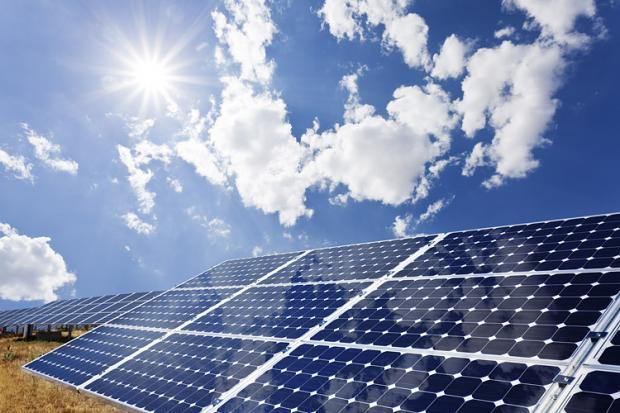
\includegraphics[width=\linewidth]{Titelbild.jpg}
\end{figure}
\vfill

{
\renewcommand\arraystretch{2}
\begin{center}
\begin{tabular}{>{\bf}p{4cm} l}
Hochschule                 &    Hochschule für Technik - FHNW\\
Studiengang                &    Elektro- und Informationstechnik\\
Autor/-en  		           & 	Mischa Knupfer, Simon Hasler\\
Dozent                   &    Pascal Schleuniger\\
Modul               &    EMV\\
Version                    &    1.0 %Normally not used!
\end{tabular}
\end{center}
}

\clearpage
			
%%---ABSTRACT----------------------------------------------------------------------------
\selectlanguage{english}				%ngerman or english
\thispagestyle{empty}
\begin{abstract}
\noindent


\end{abstract}	

%%---TABLE OF CONTENTS-------------------------------------------------------------------
\pagenumbering{Roman}		
\selectlanguage{ngerman}				%ngerman or english
\tableofcontents
\clearpage

%%---TEXT--------------------------------------------------------------------------------
\pagenumbering{arabic}
\section{Einleitung}

%Auftrag
%Was wird gemacht?
%Wie ist der Bericht aufgebaut?
\section{Schaltung}
\label{sec:Schaltung}

%Schaltung zeigen
%Funktionsweise der Schaltung
%Welche Tests sinnvoll und warum

In der Bachelor-Thesis von Simon Hasler ist eine Teilschaltung implementiert, welche den Strom eines Asynchronmotors misst. Diese Schaltung wurde von den Autoren ausgewählt, um im Modul EMV Tests durchführen zu können. Damit die Schaltung bei den Tests sicher nicht kaputt geht, sollte diese nachgebaut werden. Leider wurde bekannt, dass diese Teilschaltung, generiert von einer anderen, externen Schule, nicht funktionstüchtig ist. Aus diesem Grund haben die Autoren eine eigene Schaltung zur Strommessung mit an der Fachhochschule zur Verfügung stehenden Mitteln zusammengestellt. Bei der Schaltung handelt es sich um eine Strommessung über einen Widerstand (Shunt) mit Tiefpassfilterung und einem Operationsverstärker, zu sehen in Abbildung \ref{fig:SchaltungDraw}.\\

\begin{minipage}[b][6cm][t]{1\textwidth}
\centering
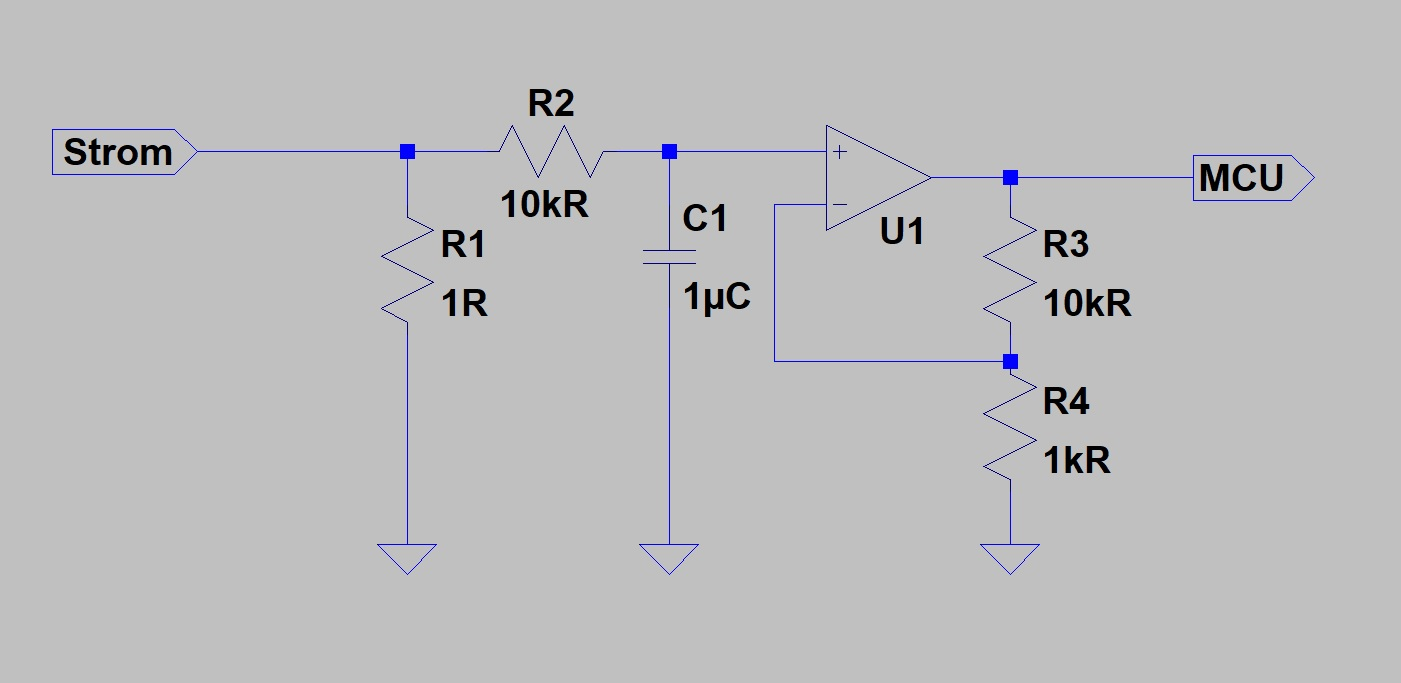
\includegraphics[angle=0,width=0.75\textwidth]{graphics/SchaltungDraw.jpg}
\captionof{figure}{Schema der entworfenen Schaltung.}
\label{fig:SchaltungDraw}
\end{minipage}
\vspace*{0.25cm}

In Abbildung \ref{fig:SchaltungDraw} ist zu sehen, dass von Links der zu messende Strom in die Schaltung hinein und durch den Shunt (R1) strömt. Ein Tiefpassfilter (R2 parallel zu C1) schützt die nachfolgende Schaltung vor Schäden durch hohe Frequenzen. Der Operationsverstärker (U1) dient als nichtinvertierender Verstärker mit einem Verstärkungsfaktor von $1+\dfrac{R3}{R4}$. Die Ausgangsspannung, welche im Verhältnis zum zu messenden Strom ist, wird an einen Mikrocontroller zur Datenverarbeitung weiteregeben (bzw. erst auf einen ADC). Der Operationsverstärker benötigt zudem eine Spannungsversorgung von +5V.\\

Das Schema wird umgesetzt mit Bauteilen, welche direkt an der Fachhochschule bezogen werden können. Ebenfalls wird nicht extra ein Print hergestellt, sondern eine Lochrasterplatine verwendet, auf welcher die Schaltung gelötet wird. Die Schaltung sieht umgesetzt aus wie in Abbildung \ref{fig:Schaltung1} aus.

\begin{minipage}[b][6cm][t]{1\textwidth}
\centering
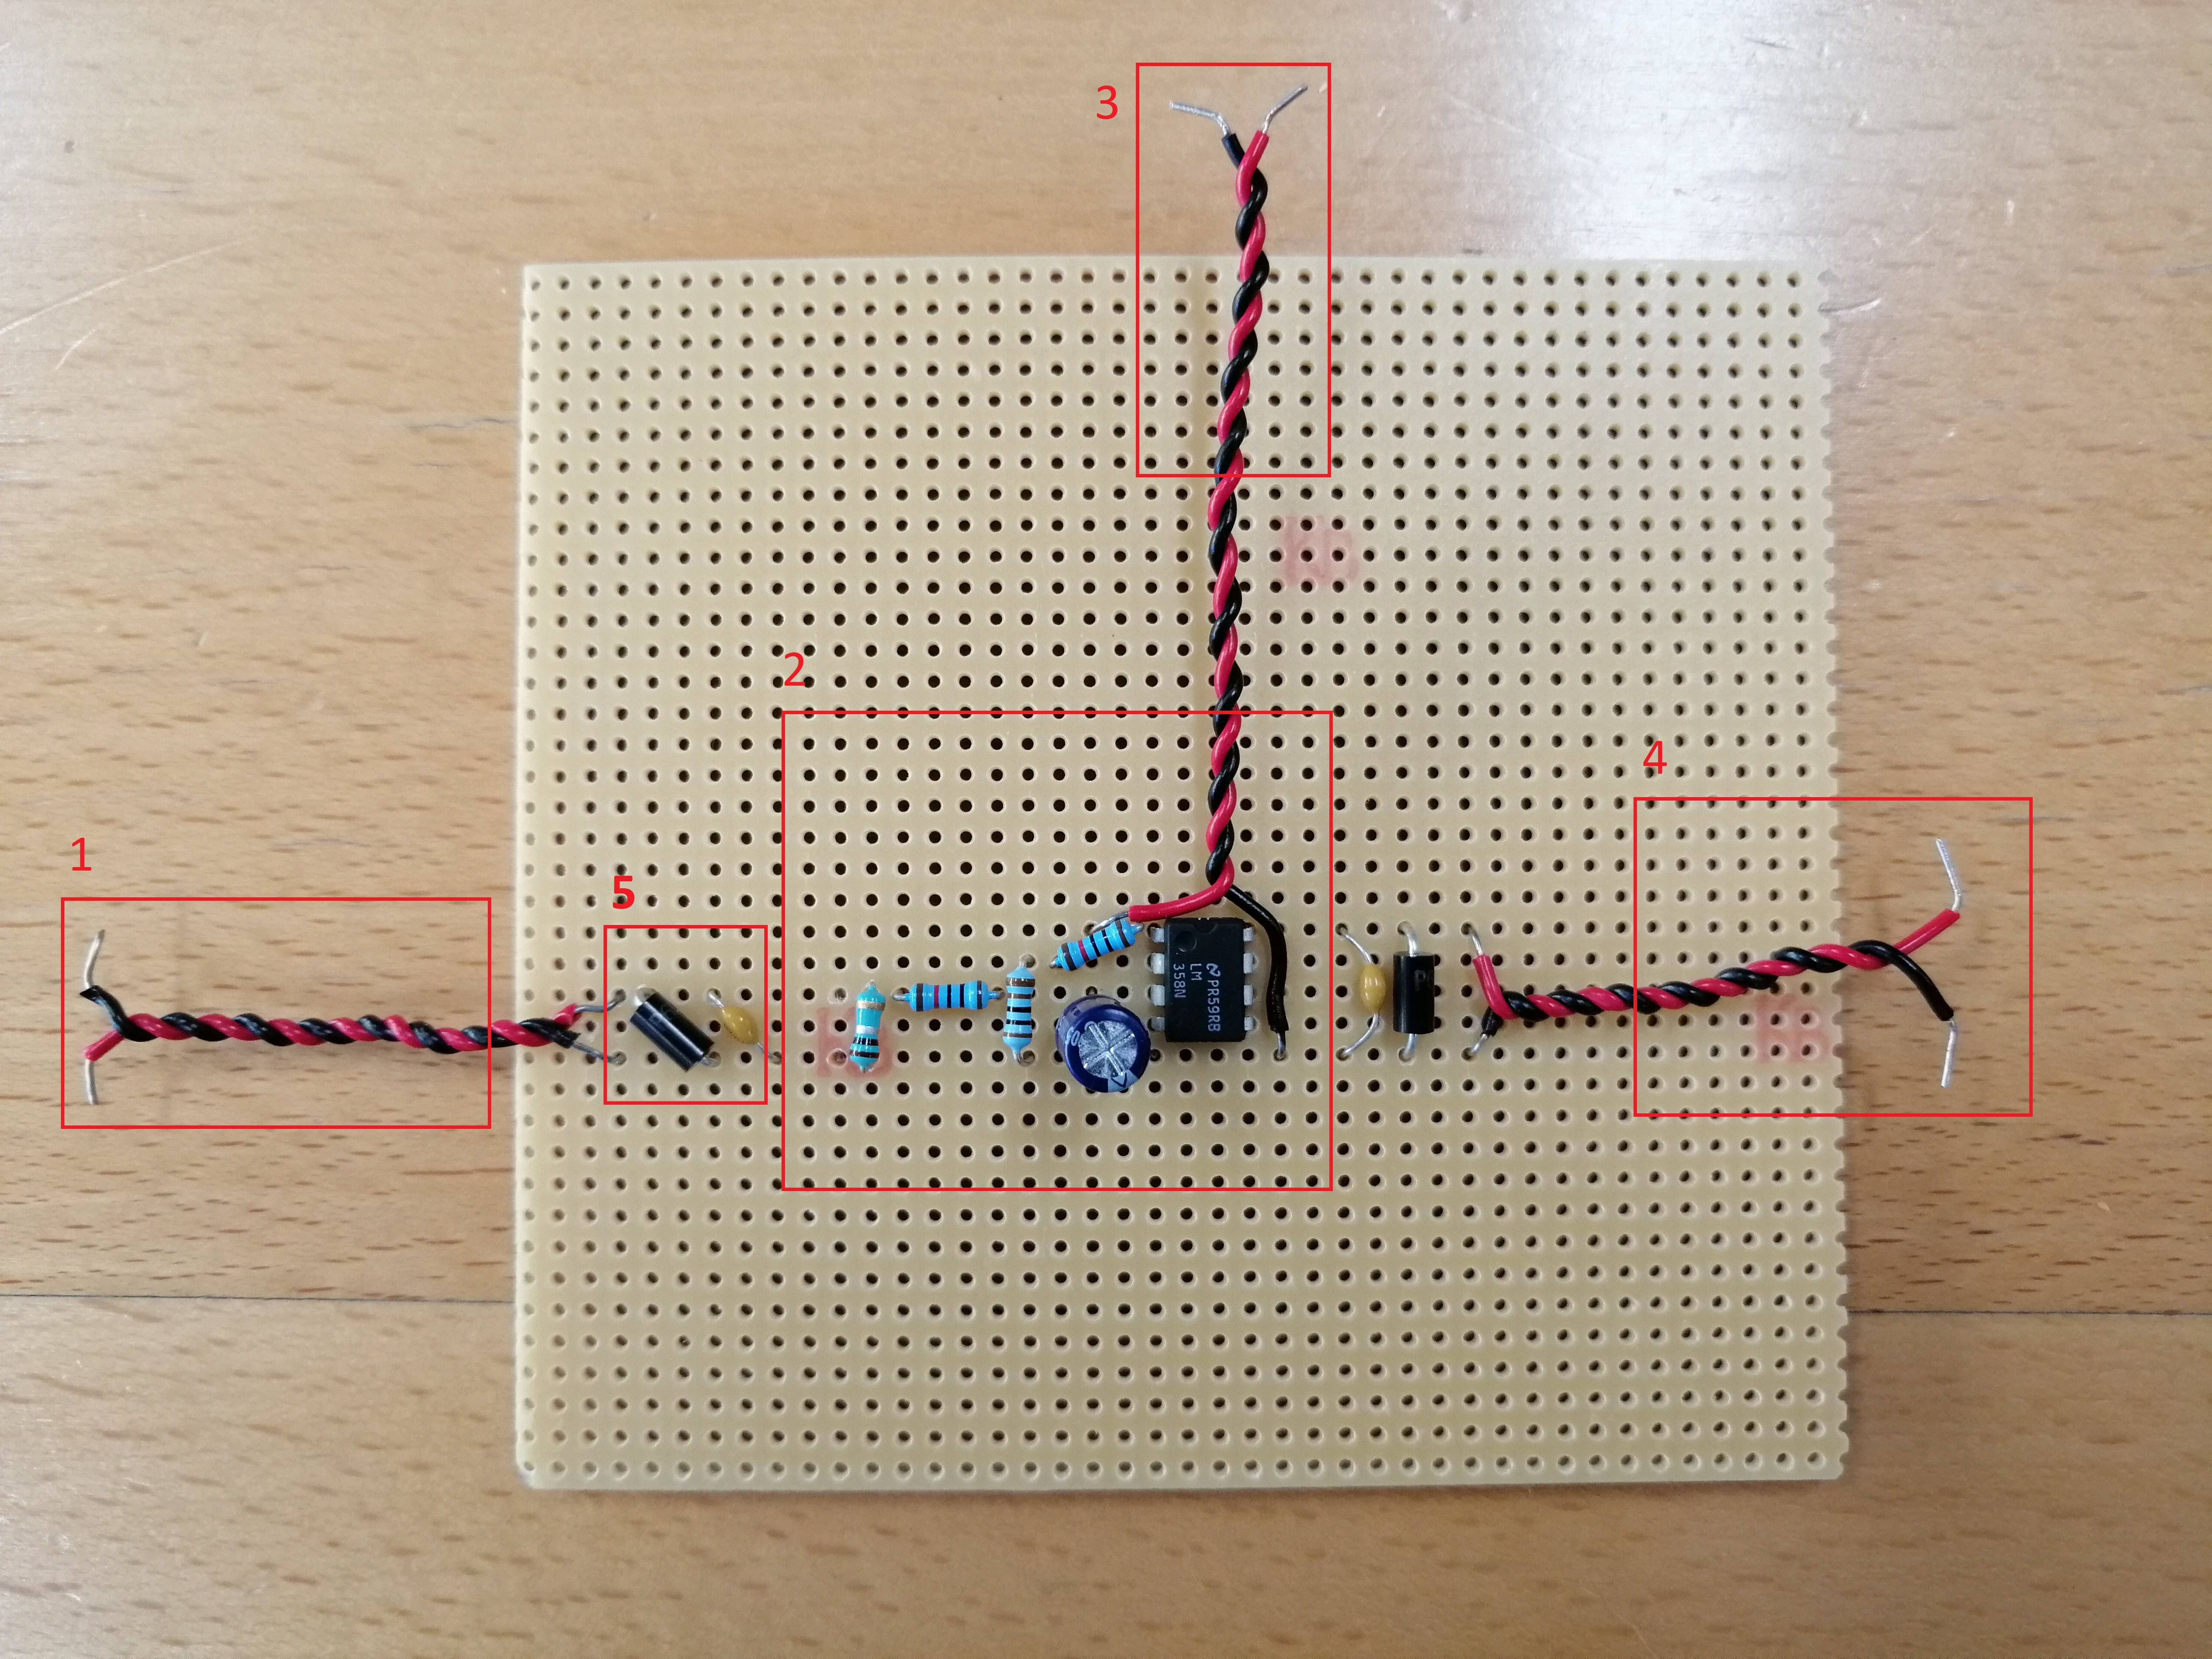
\includegraphics[angle=0,width=0.75\textwidth]{graphics/Schaltung1.jpg}
\captionof{figure}{Die realisierte entworfene Schaltung.}
\label{fig:Schaltung1}
\end{minipage}
\vspace*{4cm}

In Abbildung \ref{fig:Schaltung1} sind die Anschlüsse für eine Stromquelle (1), für den Ausgang zur MCU bzw. zum Oszilloskop (3) und für die Speisespannung des Operationsverstärkers (2) zu sehen. Die Schaltung selbst, wie in Abbildung \ref{fig:SchaltungDraw} gezeichnet, ist ebenfalls zu sehen (4). Ausserdem sind die Schutzelemente gegen die ausgewählten EMV-Störungen hier schon implementiert (5), was jedoch erst in Kapitel \ref{sec:Schutz} näher besprochen wird.\\

Damit sichergestellt ist, dass die Schaltung ihre Aufgabe erfüllt, muss dies getestet werden. Dafür wird der Ausgang an ein Oszilloskop angeschlossen, der Operationsverstärker mit einer Spannungsquelle gespiesen (5V) und am Eingang eine Stromquelle angeschlossen. Nun sollen für verschiedene Ströme auch verschiedene Spannungslevel auftreten. Die Auswertung ist zu sehen in Abbildung \ref{fig:Schaltungstest}.\\

\begin{minipage}[b][6cm][t]{1\textwidth}
\centering
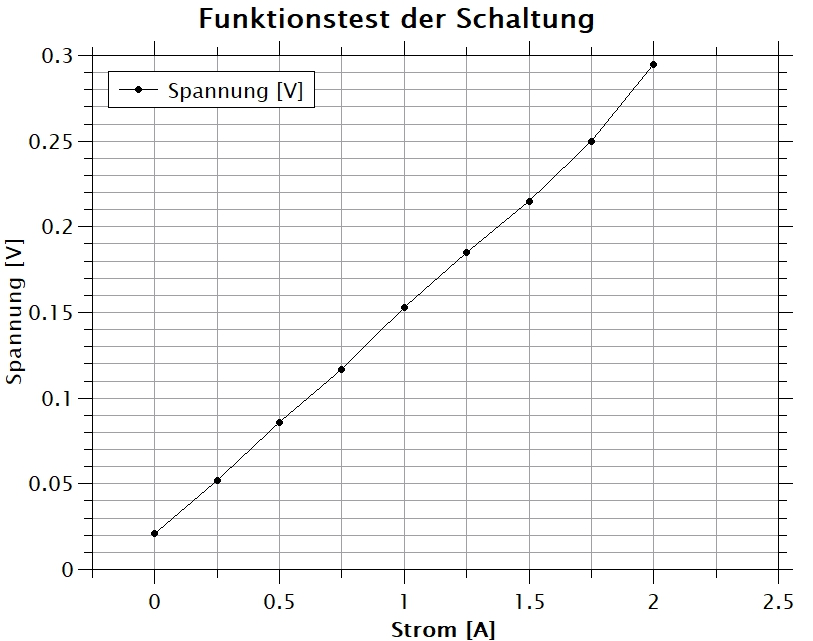
\includegraphics[angle=0,width=0.75\textwidth]{graphics/Schaltungstest.jpg}
\captionof{figure}{Das Ergebnis des Funktionstest, geplottet mit QtiPlot.}
\label{fig:Schaltungstest}
\end{minipage}
\vspace*{4cm}

Abbildung \ref{fig:Schaltungstest} zeigt die am Oszilloskop gemessene Spannung für verschiedene Eingangsströme. Es fällt ein linearer Zusammenhang auf, wobei es zu kleineren Abweichung (Messfehler, Ablesefehler...) kommt. Die Schaltung gibt also für jeden Eingangsstrom einen anderen Spannungspegel aus, weshalb gesagt werden kann, dass die Schaltung funktioniert.\\

Die Schaltung wurde aufgebaut und auf ihre Funktionalität getestet. Als nächstes folgen die ausgewählten EMV-Testarten und deren Normen, auf diese hin die Schaltung getestet wird.\\



\section{Testarten und Normen}
\label{sec:TestUndNorm}
%Welche Testarten gibt es?
%Welche sind sinnvoll bei unserer Schaltung?
\section{Schutzelemente}
\label{sec:Schutz}
%Was für Schutzelemente gibt es?
%Wie kann die Schaltung geschützt werden?

\section{Testaufbau}

%Aufzeigen was wie getestet wird und mit welchem Aufbau
\section{Testprotokoll: Burst}
\label{sec:Test:Burst}


\section{Testprotokoll: Surge}


\section{Testprotokoll: ESD}


\section{Testauswertung}
\label{sec:Auswertung}

\section{Schluss}
\label{sec:Schluss}

%Was wurde gemacht?
%Was sind die Resultate?
%Was haben wir gelernt?
%Was kann besser gemacht werden?



%%---BIBLIOGRAPHY------------------------------------------------------------------------
{\sloppypar
\printbibliography[heading=bibintoc]
\label{sec:lit}
%\selectlanguage{english}				%ngerman or english
%\printbibliography[heading=bibintoc]
}

%%---APPENDIX----------------------------------------------------------------------------
\begin{appendix}
%Anhänge

\end{appendix}

%%---NOTES for DEBUG---------------------------------------------------------------------
\ifdraft{%Do this only if mode=draft
%%requires \usepackage{todonotes})
\newpage
\listoftodos[\section{Todo-Notes}]
\clearpage
}
{%Do this only if mode=final
}
\end{document}
